\documentclass{sigchi}

% Use this command to override the default ACM copyright statement
% (e.g. for preprints).  Consult the conference website for the
% camera-ready copyright statement.

%% HOW TO OVERRIDE THE DEFAULT COPYRIGHT STRIP --
%% Please note you need to make sure the copy for your specific
%% license is used here!
% \toappear{
% Permission to make digital or hard copies of all or part of this work
% for personal or classroom use is granted without fee provided that
% copies are not made or distributed for profit or commercial advantage
% and that copies bear this notice and the full citation on the first
% page. Copyrights for components of this work owned by others than ACM
% must be honored. Abstracting with credit is permitted. To copy
% otherwise, or republish, to post on servers or to redistribute to
% lists, requires prior specific permission and/or a fee. Request
% permissions from \href{mailto:Permissions@acm.org}{Permissions@acm.org}. \\
% \emph{CHI '16},  May 07--12, 2016, San Jose, CA, USA \\
% ACM xxx-x-xxxx-xxxx-x/xx/xx\ldots \$15.00 \\
% DOI: \url{http://dx.doi.org/xx.xxxx/xxxxxxx.xxxxxxx}
% }

% Arabic page numbers for submission.  Remove this line to eliminate
% page numbers for the camera ready copy
% \pagenumbering{arabic}

% Load basic packages
\usepackage{balance}       % to better equalize the last page
\usepackage{graphics}      % for EPS, load graphicx instead 
\usepackage[T1]{fontenc}   % for umlauts and other diaeresis
\usepackage{txfonts}
\usepackage{mathptmx}
\usepackage[pdflang={en-US},pdftex]{hyperref}
\usepackage{color}
\usepackage{booktabs}
\usepackage{textcomp}

% Some optional stuff you might like/need.
\usepackage{microtype}        % Improved Tracking and Kerning
% \usepackage[all]{hypcap}    % Fixes bug in hyperref caption linking
\usepackage{ccicons}          % Cite your images correctly!
% \usepackage[utf8]{inputenc} % for a UTF8 editor only
\usepackage{subfig}

% If you want to use todo notes, marginpars etc. during creation of
% your draft document, you have to enable the "chi_draft" option for
% the document class. To do this, change the very first line to:
% "\documentclass[chi_draft]{sigchi}". You can then place todo notes
% by using the "\todo{...}"  command. Make sure to disable the draft
% option again before submitting your final document.
\usepackage{todonotes}

% Paper metadata (use plain text, for PDF inclusion and later
% re-using, if desired).  Use \emtpyauthor when submitting for review
% so you remain anonymous.
\def\plaintitle{SIGCHI Conference Proceedings Format}
\def\plainauthor{First Author, Second Author, Third Author,
  Fourth Author, Fifth Author, Sixth Author}
\def\emptyauthor{}
\def\plainkeywords{Authors' choice; of terms; separated; by
  semicolons; include commas, within terms only; required.}
\def\plaingeneralterms{Documentation, Standardization}

% llt: Define a global style for URLs, rather that the default one
\makeatletter
\def\url@leostyle{%
  \@ifundefined{selectfont}{
    \def\UrlFont{\sf}
  }{
    \def\UrlFont{\small\bf\ttfamily}
  }}
\makeatother
\urlstyle{leo}

% To make various LaTeX processors do the right thing with page size.
\def\pprw{8.5in}
\def\pprh{11in}
\special{papersize=\pprw,\pprh}
\setlength{\paperwidth}{\pprw}
\setlength{\paperheight}{\pprh}
\setlength{\pdfpagewidth}{\pprw}
\setlength{\pdfpageheight}{\pprh}

% Make sure hyperref comes last of your loaded packages, to give it a
% fighting chance of not being over-written, since its job is to
% redefine many LaTeX commands.
\definecolor{linkColor}{RGB}{6,125,233}
\hypersetup{%
  pdftitle={\plaintitle},
% Use \plainauthor for final version.
%  pdfauthor={\plainauthor},
  pdfauthor={\emptyauthor},
  pdfkeywords={\plainkeywords},
  pdfdisplaydoctitle=true, % For Accessibility
  bookmarksnumbered,
  pdfstartview={FitH},
  colorlinks,
  citecolor=black,
  filecolor=black,
  linkcolor=black,
  urlcolor=linkColor,
  breaklinks=true,
  hypertexnames=false
}

% create a shortcut to typeset table headings
% \newcommand\tabhead[1]{\small\textbf{#1}}

% End of preamble. Here it comes the document.
\begin{document}

\title{Multi-Instance Learning for Coarsely Labeled Time-Domain Inference}

\numberofauthors{3}
\author{%
  \alignauthor{Leave Authors Anonymous\\
    \affaddr{for Submission}\\
    \affaddr{City, Country}\\
    \email{e-mail address}}\\
  \alignauthor{Leave Authors Anonymous\\
    \affaddr{for Submission}\\
    \affaddr{City, Country}\\
    \email{e-mail address}}\\
  \alignauthor{Leave Authors Anonymous\\
    \affaddr{for Submission}\\
    \affaddr{City, Country}\\
    \email{e-mail address}}\\
}

\maketitle

\begin{abstract}
  In the supervised learning setting, it is essential to have sufficient labeled data; however, in many domains, such as activity recognition, existing labeled data may not be available and the annotation process is often too cumbersome, time-consuming and prone to human error. In this work, we explore the use of Multiple-Instance Learning (MIL) in order to reduce the need for fine-grained labels. We examine the drop in performance on two existing time-domain gesture-annotated datasets and show that MIL given coarse-grain ground-truth annotations can achieve performance metrics comparable with standard supervised Machine Learning approaches given fine-grain labels. We evaluate the performance in a leave-one-participant-out fashion given (1) coarsely labeled field data, (2) finely labeled lab data and (3) coarsely labeled data from the held-out participant. Our analysis shows that we can achieve competitive performance given a small number of fine-grained labels in addition to many coarse-grained labels and that even very few labeled sessions from the held-out participant improve performance significantly. We use this to design a system that gives recommendations to developers on the granularity of the field data, based on an initial lab dataset.
\end{abstract}

\category{H.5.m.}{Information Interfaces and Presentation
  (e.g. HCI)}{Miscellaneous} \category{See
  \url{http://acm.org/about/class/1998/} for the full list of ACM
  classifiers. This section is required.}{}{}

\keywords{Multi-Instance Learning; Data Collection; Time-Domain; Activity Recognition; Eating Detection; Smoking Detection}

\section{Introduction}

The ubiquity of mobile devices has led to a growing body of research in designing and solving gesture recognition tasks. These efforts have enormous implications in the mobile health community, self-tracking fitness industry and the development of state-of-the-art human-computer interfacing. The standard approach to gestural recognition employs an appropriate supervised classifier, which often performs exceptionally well given large amounts of labeled data and a well-chosen feature representation. The bottleneck to this approach is that acquiring sufficient gesture labels may be challenging, time-consuming or costly. While many techniques have been adopted to reduce the data annotation effort, this often comes at the expense of noisy labels due to factors such as human error.

A commonly used lightweight approach to gesture annotation is experience sampling [-1], where human subjects are prompted to label their current activity or recount their previous activity break-down. This is often best suited when the activities span a large enough time interval; otherwise, acquiring fine-grained labels remains difficult and especially prone to human error.

One of the most common solutions to reduce human error in data collection is video annotation. Although video labeling is relatively robust to human error, it is time-consuming, it introduces privacy concerns, and its power consumption is significantly large, making it impractical for collecting large-scale data in the field. Thus, there has been a significant effort to reduce the use of video recordings for annotated data collection while minimizing the label noise. Thomaz et al. [-1] employ an upward-facing camera mounted on a necklace to capture eating gestures in the field; the camera takes a snapshot of the subject every 30 seconds, significantly reducing the power consumption and labeling efforts required. Parate et al. [-1] use a 6-axis inertial sensor equipped on the upper arm in addition to a wrist-worn sensor in order to visualize the arm movements in a virtual 3D environment. This eliminates the need for video recordings while minimally increasing the risk of error. However, the annotation effort remains cumbersome and does not scale well to field data, because the additional armband is obtrusive.

Trabelsi et al. [-1] eliminate the need for training data altogether by using an unsupervised learning approach based on a Hidden Markov Model. While this technique achieves performance comparable to supervised learning approaches, it only provides a partition of the data by class and does not make precise label predictions in the absence of labeled data. When a large number of classes are present or positive labels are sparse, then sufficient annotated data once again becomes essential to realize robust, deployable classification systems.

Recent work by Stikic and Schiele [-1] explores the feasibility of using Multi-Instance Learning (MIL) to reduce the labeling effort of activity recognition tasks while incurring minimal additional classification error. Although they show that comparable performance can be achieved with coarse-grained labels, they do not consider the case when the developers provide a small number of fine-grained labels in addition to field data.

In this work we demonstrate the on time-domain inertial data and evaluate the extent to which session-level and gesture-level labels improve performance. We additionally assess the boost in performance given a small number of fine-grained labels from the test user in a leave-one-participant-out evaluation. The

\section{Multi-Instance Learning}

In the Multi-Instance Learning (MIL) framework, we jointly consider instances, the atomic units over which predictions are made (i.e. gestures), and bags of instances, which may correspond to sessions or longer, manageable time intervals over which an activity is performed. In the binary setting, each bag is assigned a positive label if at least one instance in the bag is positive; bags with no positive instances are assumed to be negative.

The most naive MIL approach is Single-Instance Learning (SIL) [-1], which makes the usually false assumption that every instance in a positive bag is positive. This reduces the problem to a supervised instance-level classification task, which is generally done using a Support Vector Machine (SVM). When positive instances are sparse, the SIL assumption significantly hurts the classification performance.

In the activity recognition setting, Stikic and Schiele use the Maximum Pattern Margin Formulation (miSVM) originally proposed by Andrews et al. [-1] in order to account for the sparsity of positive bags. Due to the non-convexity of the objective function, they use a heuristic to learn the separating hyperplane. They initially train an SIL SVM, whose decision hyperplane is used to relabel the most positive predictions within positive bags. The SVM is then retrained on the relabeled data and the process is repeated until the labels converge. Although this approach accounts for the sparsity of positive gestures, it tends to over-predict the positive class [?] and has no mechanism to adjust the sensitivity based on known density.

Bunescu and Mooney [-1] deal with the challenge of sparse positive bags by using an adaptive SVM constraint (sMIL). In particular, they formulate the MIL constraint that there exists at least one positive instance in every positive bag $X$ as follows

\begin{align*}
	w \frac{\phi(X)}{\left| X \right|} + b \geq \frac{2 - \left| X \right|}{\left| X \right|} - \xi_X \\
	\xi_X \geq 0
\end{align*}

where $w \frac{\phi(X)}{\left| X \right|} + b$ is the normalized prediction scores under the feature function $\phi$, weights $w$ and bias $b$, and $\xi_X$ is the non-negative slack parameter that allows some extent of misclassification of instances in $X$ to avoid over-fitting the model to the training data. When the bag size $\left| X \right|$ is small, the right-hand side becomes larger, suggesting that smaller positive bags are more informative.

Bunescu and Mooney additionally introduce a balancing parameter $\eta$, indicating the expected class distribution of instances within bags. The sparse balancing MIL (sbMIL) approach initially trains a sMIL classifier, then relabels the $\eta \left| X \right|$ most positive instances as positive and the remaining instances as negative. The final hyperplane is then learned using SIL given the relabeled data.

In this work we employ the sbMIL due to the sparsity of positive labels.

\section{Data}

In order to reason in a practical sense about the trade-off between performance and labeling effort under the MIL formulation, we perform several evaluations on two existing datasets: the lab-20 eating dataset developed by Edison Thomaz [-1] and the RisQ smoking dataset developed by Parate et al. [-1]. In order to assess how well the model generalizes to unseen users, we perform leave-one-participant-out (LOPO) evaluations; that is, the model is trained on all but one participant and then evaluated on the held out participant.

\subsection{Lab-20 Eating}

The lab-20 eating dataset comprises of 25Hz 3-axis accelerometer data collected using a wrist-worn inertial sensor from 20 individuals. Individuals were provided food to eat and were asked to perform other possible confounding actions as they please, including talking on the phone, brushing their teeth and combing their hair. The average duration across participants is 31 minutes 21 seconds and comprises of approximately 48\% eating sessions. Note, however, that the proportion of eating gestures is much smaller, since non-eating gestures are frequently present within eating sessions.

We use Thomaz's evaluation as the baseline result for comparison. In his work, he uses a Random Forest classifier over 15 statistical features (mean, variance, skew, kurtosis and root mean square over each axis) extracted over windows of 6 seconds with 50\% overlap. He reports a 0.42 average LOPO f1 score. We achieve similar performance using a linear SVM.

\subsection{RisQ Dataset}

The RisQ smoking dataset contains 50Hz fused 9-axis inertial data in the form of quaternions from 15 subjects. Parate reports a precision of 91\% and recall of 81\%. The pipeline consists of (1) computing the trajectory from the quaternion stream, (2) identifying candidate windows by locating peak-trough-peak patterns, (3) extracting 37 angle, velocity, displacement and duration features, (4) classifying windows using a Random Forest and (5) smoothing the predictions using a Conditional Random Field.

In our work, we use the same pipeline but replace the Random Forest classifier with a sbMIL classifier to allow for sparse labels.

\begin{figure}
\centering
  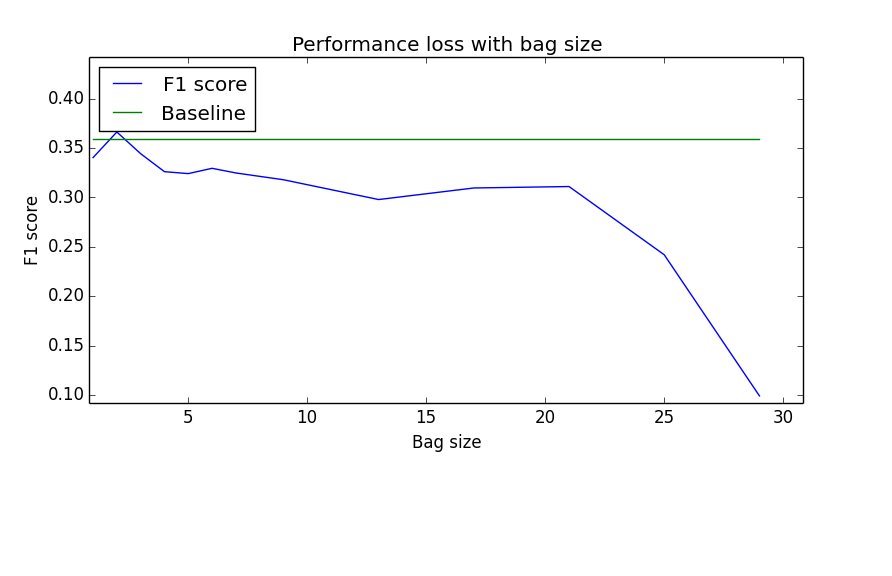
\includegraphics[width=0.9\columnwidth]{figures/sbMIL_bag_size2}
  \caption{Average LOPO f1 score of sbMIL on Lab-20 dataset as a function of the bag size}~\label{fig:figure1}
\end{figure}

\section{Experimental Setup}

\begin{figure*}
  \centering
  \subfloat[M = 150]{{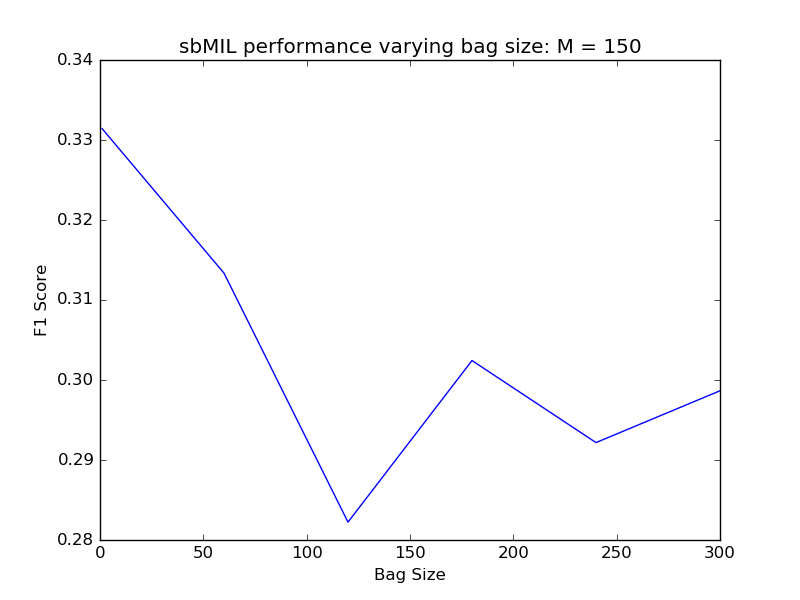
\includegraphics[width=5cm]{figures/_M150} }}%
  \qquad
  \subfloat[M = 300]{{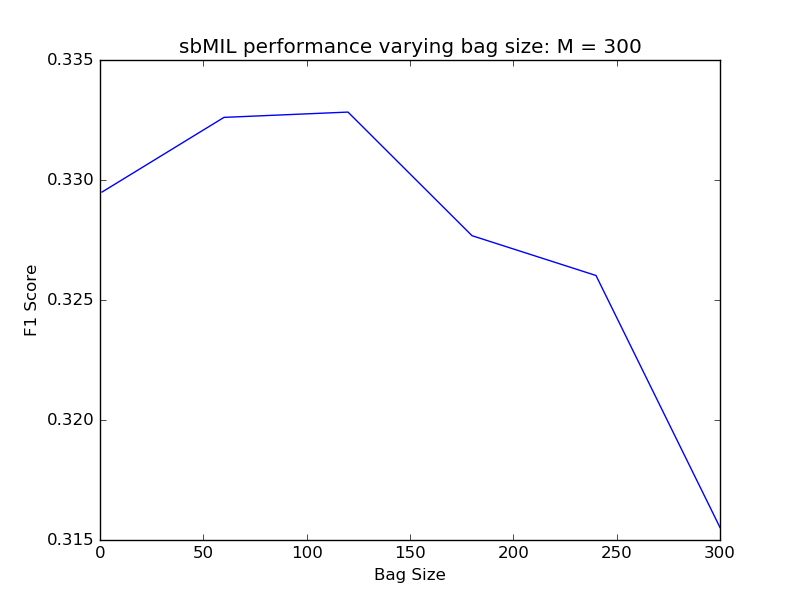
\includegraphics[width=5cm]{figures/_M300} }}%
  \qquad
  \subfloat[M = 450]{{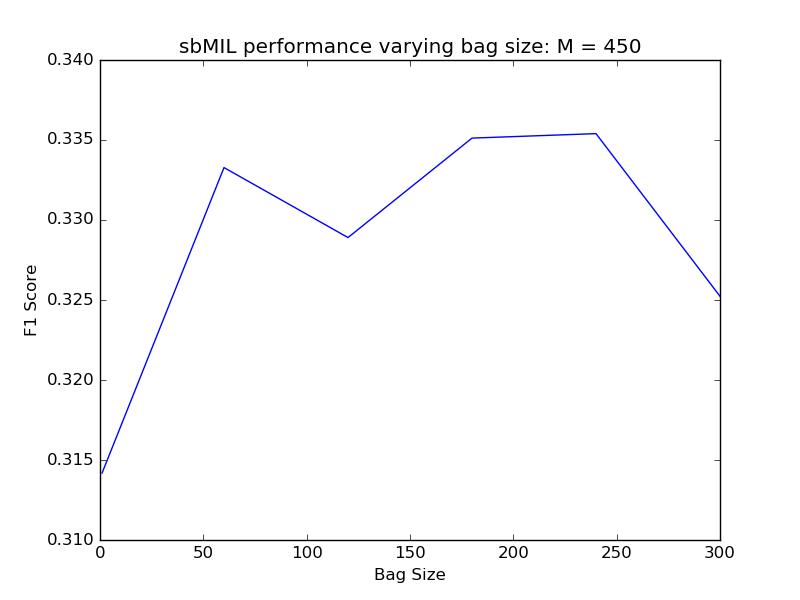
\includegraphics[width=5cm]{figures/_M450} }}%
  \caption{Average LOPO performance of sbMIL on Lab-20 dataset as a function of the bag size given 150, 300 and 450 additional labeled training instances respectively }~\label{fig:figure2}
\end{figure*}

In order to reason about the effectiveness of MIL techniques in gesture recognition, we evaluate the average LOPO performance for various bag sizes. Figure \ref{fig:figure1} shows for the Lab-20 eating dataset that as the bag size decreases, the performance of each MIL technique drops, and it is upper bounded by the baseline SVM performance.

Evidently, the performance is greater given more finely-grained labels. However, given that these labels may be difficult to acquire, we must ask: How many such labels do we need?

In order to address this, we evaluate several experiments in which $M$ fine-grained labels are provided by 5 participants and $N$ coarse-grained labels are provided by the remaining 14 participants. The coarse-grained labels may either be labeled sessions, which may vary in duration, or partitions of the data with a fixed duration. As a personalization step for enhancing performance, we additionally include $K$ instances from the held-out participant in the training data, which are then excluded from the test set. Our experiments involve varying the values of $N$, $M$ and $K$.

In each of the experiments, a subset of the training data is used and is therefore selected uniformly from the entire training data; to smooth out noise introduced by the randomness, the performance is averaged over 10 trials. The performance reported is in each case the best performance achieved using cross-validation over the model hyperparameters. These parameters include the expected class weights, the sparse balancing parameter $\eta$ and the SVM regularization constant $C$.

\section{Evaluation}

\subsection{Lab-20 Eating}

From figure \ref{fig:figure1} it is clear that the performance drops very quickly as the granularity of the labels decreases. However, figure \ref{fig:figure2} demonstrates that this drop in performance is minimal even for large bag sizes, if in additional to coarse labels, fine grained labels are provided. This is shown when 150, 300 or 450 labeled training instances are provided from the lab data. When $M = 450$, the performance remains roughly the same, meaning it may be acceptable to use field data with bag sizes of up to 300.

\begin{figure*}
  \centering
  \subfloat[bag size : 15 (1 min 30 s)]{{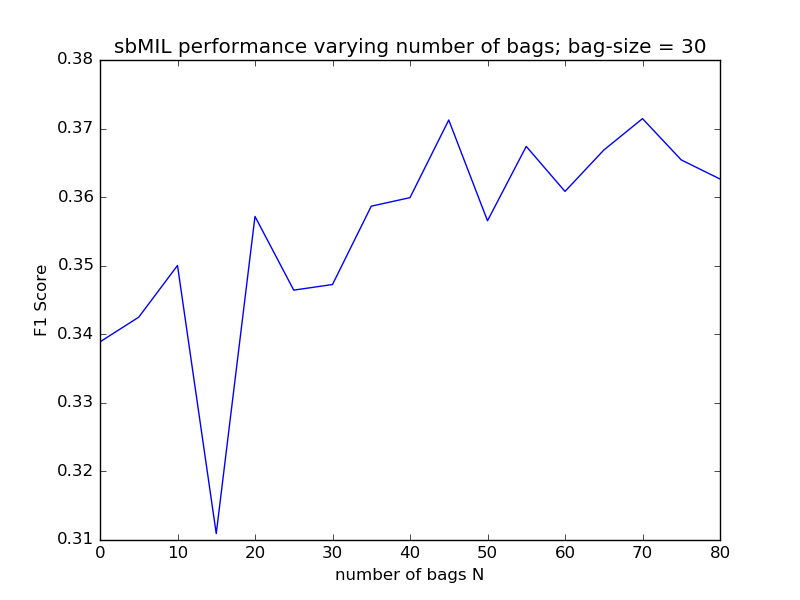
\includegraphics[width=5cm]{figures/_b30} }}%
  \qquad
  \subfloat[bag size : 150 (15 min)]{{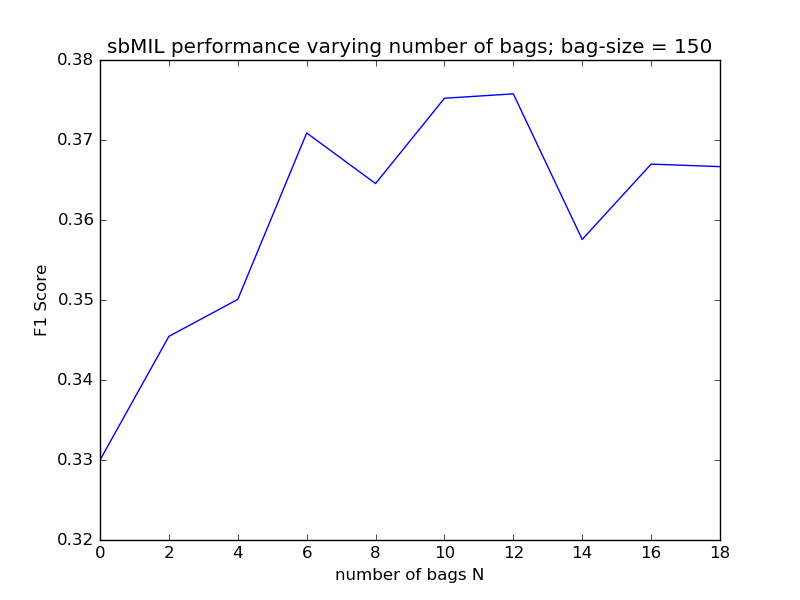
\includegraphics[width=5cm]{figures/_b150} }}%
  \qquad
  \subfloat[bag size : 300 (30 min)]{{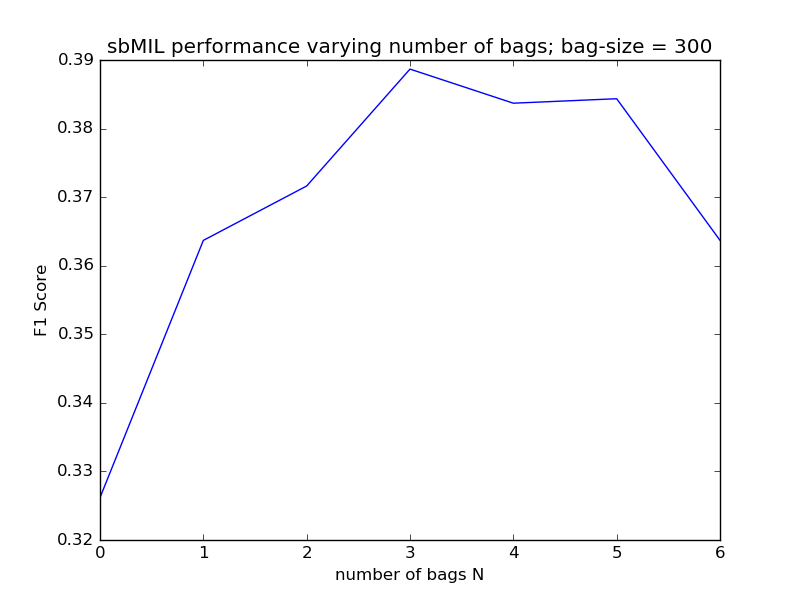
\includegraphics[width=5cm]{figures/_b300} }}%
  \caption{Average LOPO performance of sbMIL on Lab-20 dataset as a function of the number of bags given bag sizes of 15, 150 and 300 respectively}~\label{fig:figure3}
\end{figure*}

Figure \ref{fig:figure3} shows the average LOPO performance on the Lab-20 eating dataset as the number of bags increases for bag sizes of 15, 150 and 300 instances. These correspond roughly to 1.5, 15 and 30 minute bags respectively. As the amount of training data increases, the f1 score increases, as expected. Interestingly, the performance is greater given larger bags, even when fewer labels are available. This suggests that many unlabeled instances are preferable to few labeled instances. This is the essential advantage of using MIL techniques.

\subsection{RisQ Dataset}

In the RisQ dataset

\section{Typeset Text}
The styles contained in this document have been modified from the
default styles to reflect ACM formatting conventions. For example,
content paragraphs like this one are formatted using the Normal style.

\LaTeX\ sometimes will create overfull lines that extend into columns.
To attempt to combat this, the \texttt{.cls} file has a command,
\texttt{{\textbackslash}sloppy}, that essentially asks \LaTeX\ to
prefer underfull lines with extra whitespace.  For more details on
this, and info on how to control it more finely, check out
{\url{http://www.economics.utoronto.ca/osborne/latex/PMAKEUP.HTM}}.

\subsection{References and Citations}

Use a numbered list of references at the end of the article, ordered
alphabetically by last name of first author, and referenced by numbers
in
brackets~\cite{acm_categories,ethics,Klemmer:2002:WSC:503376.503378}.
Your references should be published materials accessible to the
public. Internal technical reports may be cited only if they are
easily accessible (i.e., you provide the address for obtaining the
report within your citation) and may be obtained by any reader for a
nominal fee. Proprietary information may not be cited. Private
communications should be acknowledged in the main text, not referenced
(e.g., ``[Borriello, personal communication]'').

References should be in ACM citation format:
\url{http://acm.org/publications/submissions/latex_style}. This
includes citations to internet
resources~\cite{acm_categories,cavender:writing,CHINOSAUR:venue,psy:gangnam}
according to ACM format, although it is often appropriate to include
URLs directly in the text, as above.


% Use a numbered list of references at the end of the article, ordered
% alphabetically by first author, and referenced by numbers in
% brackets~\cite{ethics, Klemmer:2002:WSC:503376.503378,
%   Mather:2000:MUT, Zellweger:2001:FAO:504216.504224}. For papers from
% conference proceedings, include the title of the paper and an
% abbreviated name of the conference (e.g., for Interact 2003
% proceedings, use \textit{Proc. Interact 2003}). Do not include the
% location of the conference or the exact date; do include the page
% numbers if available. See the examples of citations at the end of this
% document. Within this template file, use the \texttt{References} style
% for the text of your citation.

% Your references should be published materials accessible to the
% public.  Internal technical reports may be cited only if they are
% easily accessible (i.e., you provide the address for obtaining the
% report within your citation) and may be obtained by any reader for a
% nominal fee.  Proprietary information may not be cited. Private
% communications should be acknowledged in the main text, not referenced
% (e.g., ``[Robertson, personal communication]'').

\begin{table}
  \centering
  \begin{tabular}{l r r r}
    % \toprule
    & & \multicolumn{2}{c}{\small{\textbf{Test Conditions}}} \\
    \cmidrule(r){3-4}
    {\small\textit{Name}}
    & {\small \textit{First}}
      & {\small \textit{Second}}
    & {\small \textit{Final}} \\
    \midrule
    Marsden & 223.0 & 44 & 432,321 \\
    Nass & 22.2 & 16 & 234,333 \\
    Borriello & 22.9 & 11 & 93,123 \\
    Karat & 34.9 & 2200 & 103,322 \\
    % \bottomrule
  \end{tabular}
  \caption{Table captions should be placed below the table. We
    recommend table lines be 1 point, 25\% black. Minimize use of
    table grid lines.}~\label{tab:table1}
\end{table}

\section{Sections}

The heading of a section should be in Helvetica or Arial 9-point bold,
all in capitals. Sections should \textit{not} be numbered.

\subsection{Subsections}

Headings of subsections should be in Helvetica or Arial 9-point bold
with initial letters capitalized.  For sub-sections and
sub-subsections, a word like \emph{the} or \emph{of} is not
capitalized unless it is the first word of the heading.

\subsubsection{Sub-subsections}

Headings for sub-subsections should be in Helvetica or Arial 9-point
italic with initial letters capitalized.  Standard
\texttt{{\textbackslash}section}, \texttt{{\textbackslash}subsection},
and \texttt{{\textbackslash}subsubsection} commands will work fine in
this template.

\section{Figures/Captions}

Place figures and tables at the top or bottom of the appropriate
column or columns, on the same page as the relevant text (see
Figure~\ref{fig:figure1}). A figure or table may extend across both
columns to a maximum width of 17.78 cm (7 in.).

Captions should be Times New Roman or Times Roman 9-point bold.  They
should be numbered (e.g., ``Table~\ref{tab:table1}'' or
``Figure~\ref{fig:figure1}''), centered and placed beneath the figure
or table.  Please note that the words ``Figure'' and ``Table'' should
be spelled out (e.g., ``Figure'' rather than ``Fig.'') wherever they
occur. Figures, like Figure~\ref{fig:figure2}, may span columns and
all figures should also include alt text for improved accessibility.
Papers and notes may use color figures, which are included in the page
limit; the figures must be usable when printed in black-and-white in
the proceedings.

The paper may be accompanied by a short video figure up to five
minutes in length. However, the paper should stand on its own without
the video figure, as the video may not be available to everyone who
reads the paper.  

\subsection{Inserting Images}
When possible, include a vector formatted graphic (i.e. PDF or EPS).
When including bitmaps,  use an image editing tool to resize the image
at the appropriate printing resolution (usually 300 dpi).

\section{Quotations}
Quotations may be italicized when \textit{``placed inline''} (Anab,
23F).

\begin{quote}
Longer quotes, when placed in their own paragraph, need not be
italicized or in quotation marks when indented (Ramon, 39M).  
\end{quote}

\section{Language, Style, and Content}

The written and spoken language of SIGCHI is English. Spelling and
punctuation may use any dialect of English (e.g., British, Canadian,
US, etc.) provided this is done consis- tently. Hyphenation is
optional. To ensure suitability for an international audience, please
pay attention to the following:

\begin{itemize}
\item Write in a straightforward style.
\item Try to avoid long or complex sentence structures.
\item Briefly define or explain all technical terms that may be
  unfamiliar to readers.
\item Explain all acronyms the first time they are used in your
  text---e.g., ``Digital Signal Processing (DSP)''.
\item Explain local references (e.g., not everyone knows all city
  names in a particular country).
\item Explain ``insider'' comments. Ensure that your whole audience
  understands any reference whose meaning you do not describe (e.g.,
  do not assume that everyone has used a Macintosh or a particular
  application).
\item Explain colloquial language and puns. Understanding phrases like
  ``red herring'' may require a local knowledge of English.  Humor and
  irony are difficult to translate.
\item Use unambiguous forms for culturally localized concepts, such as
  times, dates, currencies, and numbers (e.g., ``1--5--97'' or
  ``5/1/97'' may mean 5 January or 1 May, and ``seven o'clock'' may
  mean 7:00 am or 19:00). For currencies, indicate equivalences:
  ``Participants were paid {\fontfamily{txr}\selectfont \textwon}
  25,000, or roughly US \$22.''
\item Be careful with the use of gender-specific pronouns (he, she)
  and other gendered words (chairman, manpower, man-months). Use
  inclusive language that is gender-neutral (e.g., she or he, they,
  s/he, chair, staff, staff-hours, person-years). See the
  \textit{Guidelines for Bias-Free Writing} for further advice and
  examples regarding gender and other personal
  attributes~\cite{Schwartz:1995:GBF}. Be particularly aware of
  considerations around writing about people with disabilities.
\item If possible, use the full (extended) alphabetic character set
  for names of persons, institutions, and places (e.g.,
  Gr{\o}nb{\ae}k, Lafreni\'ere, S\'anchez, Nguy{\~{\^{e}}}n,
  Universit{\"a}t, Wei{\ss}enbach, Z{\"u}llighoven, \r{A}rhus, etc.).
  These characters are already included in most versions and variants
  of Times, Helvetica, and Arial fonts.
\end{itemize}

\section{Accessibility}
The Executive Council of SIGCHI has committed to making SIGCHI
conferences more inclusive for researchers, practitioners, and
educators with disabilities. As a part of this goal, the all authors
are asked to work on improving the accessibility of their
submissions. Specifically, we encourage authors to carry out the
following five steps:
\begin{enumerate}
\item Add alternative text to all figures
\item Mark table headings
\item Add tags to the PDF
\item Verify the default language
\item Set the tab order to ``Use Document Structure''
\end{enumerate}
For more information and links to instructions and resources, please
see: \url{http://chi2016.acm.org/accessibility}.  The
\texttt{{\textbackslash}hyperref} package allows you to create well tagged PDF files,
please see the preamble of this template for an example.

\section{Page Numbering, Headers and Footers}
Your final submission should not contain footer or header information
at the top or bottom of each page. Specifically, your final submission
should not include page numbers. Initial submissions may include page
numbers, but these must be removed for camera-ready. Page numbers will
be added to the PDF when the proceedings are assembled.

\section{Producing and Testing PDF Files}

We recommend that you produce a PDF version of your submission well
before the final deadline.  Your PDF file must be ACM DL
Compliant. The requirements for an ACM Compliant PDF are available at:
{\url{http://www.sheridanprinting.com/typedept/ACM-distilling-settings.htm}}.

Test your PDF file by viewing or printing it with the same software we
will use when we receive it, Adobe Acrobat Reader Version 10. This is
widely available at no cost. Note that most
reviewers will use a North American/European version of Acrobat
reader, so please check your PDF accordingly.

When creating your PDF from Word, ensure that you generate a tagged
PDF from improved accessibility. This can be done by using the Adobe
PDF add-in, also called PDFMaker. Select Acrobat | Preferences from
the ribbon and ensure that ``Enable Accessibility and Reflow with
tagged Adobe PDF'' is selected. You can then generate a tagged PDF by
selecting ``Create PDF'' from the Acrobat ribbon.

\section{Conclusion}

It is important that you write for the SIGCHI audience. Please read
previous years' proceedings to understand the writing style and
conventions that successful authors have used. It is particularly
important that you state clearly what you have done, not merely what
you plan to do, and explain how your work is different from previously
published work, i.e., the unique contribution that your work makes to
the field. Please consider what the reader will learn from your
submission, and how they will find your work useful. If you write with
these questions in mind, your work is more likely to be successful,
both in being accepted into the conference, and in influencing the
work of our field.

\section{Acknowledgments}

Sample text: We thank all the volunteers, and all publications support
and staff, who wrote and provided helpful comments on previous
versions of this document. Authors 1, 2, and 3 gratefully acknowledge
the grant from NSF (\#1234--2012--ABC). \textit{This whole paragraph is
  just an example.}

% Balancing columns in a ref list is a bit of a pain because you
% either use a hack like flushend or balance, or manually insert
% a column break.  http://www.tex.ac.uk/cgi-bin/texfaq2html?label=balance
% multicols doesn't work because we're already in two-column mode,
% and flushend isn't awesome, so I choose balance.  See this
% for more info: http://cs.brown.edu/system/software/latex/doc/balance.pdf
%
% Note that in a perfect world balance wants to be in the first
% column of the last page.
%
% If balance doesn't work for you, you can remove that and
% hard-code a column break into the bbl file right before you
% submit:
%
% http://stackoverflow.com/questions/2149854/how-to-manually-equalize-columns-
% in-an-ieee-paper-if-using-bibtex
%
% Or, just remove \balance and give up on balancing the last page.
%
\balance{}

\section{References Format}
Your references should be published materials accessible to the
public. Internal technical reports may be cited only if they are
easily accessible and may be obtained by any reader for a nominal
fee. Proprietary information may not be cited. Private communications
should be acknowledged in the main text, not referenced (e.g.,
[Golovchinsky, personal communication]). References must be the same
font size as other body text. References should be in alphabetical
order by last name of first author. Use a numbered list of references
at the end of the article, ordered alphabetically by last name of
first author, and referenced by numbers in brackets. For papers from
conference proceedings, include the title of the paper and the name of
the conference. Do not include the location of the conference or the
exact date; do include the page numbers if available. 

References should be in ACM citation format:
\url{http://www.acm.org/publications/submissions/latex_style}.  This
includes citations to Internet
resources~\cite{CHINOSAUR:venue,cavender:writing,psy:gangnam}
according to ACM format, although it is often appropriate to include
URLs directly in the text, as above. Example reference formatting for
individual journal articles~\cite{ethics}, articles in conference
proceedings~\cite{Klemmer:2002:WSC:503376.503378},
books~\cite{Schwartz:1995:GBF}, theses~\cite{sutherland:sketchpad},
book chapters~\cite{winner:politics}, an entire journal
issue~\cite{kaye:puc},
websites~\cite{acm_categories,cavender:writing},
tweets~\cite{CHINOSAUR:venue}, patents~\cite{heilig:sensorama}, 
games~\cite{supermetroid:snes}, and
online videos~\cite{psy:gangnam} is given here.  See the examples of
citations at the end of this document and in the accompanying
\texttt{BibTeX} document. This formatting is a edited version of the
format automatically generated by the ACM Digital Library
(\url{http://dl.acm.org}) as ``ACM Ref.'' DOI and/or URL links are
optional but encouraged as are full first names. Note that the
Hyperlink style used throughout this document uses blue links;
however, URLs in the references section may optionally appear in
black.

% BALANCE COLUMNS
\balance{}

% REFERENCES FORMAT
% References must be the same font size as other body text.
\bibliographystyle{SIGCHI-Reference-Format}
\bibliography{sample}

\end{document}

%%% Local Variables:
%%% mode: latex
%%% TeX-master: t
%%% End:
